Deși aceste metode rezolvă aceeași problema, de a combina conținutul unei poze cu stilul alteia pentru a obține o nouă poză artistica ele pot fi aplicate în funcție de necesitatea utilizatorului. De exemplu, dacă utilizatorul dorește să combine picturi celebre atunci metoda lui Leon A. Gatys este cea mai potrivită. În schimb dacă se dorește doar combinarea unor anumite obiecte pentru obținerea unor noi rezultate interesante, atunci se poate aplica metoda lui Fujun Luan. Pentru o generare rapidă a pozelor artistice se poate apela la metoda lui Justin Johnson, metodă cu care se pot obține rezultate asemănătoare cu metoda lui Leon A. Gatys, dar care are un timp de rulare foarte mic.

Mai jos o să arăt câteva exemple pentru a evidenția îmbunătățirile aduse de ultimele două metode în comparație cu prima.

\begin{figure}[h]
	\centering
    \begin{subfigure}[b]{0.24\textwidth}
		\centering
        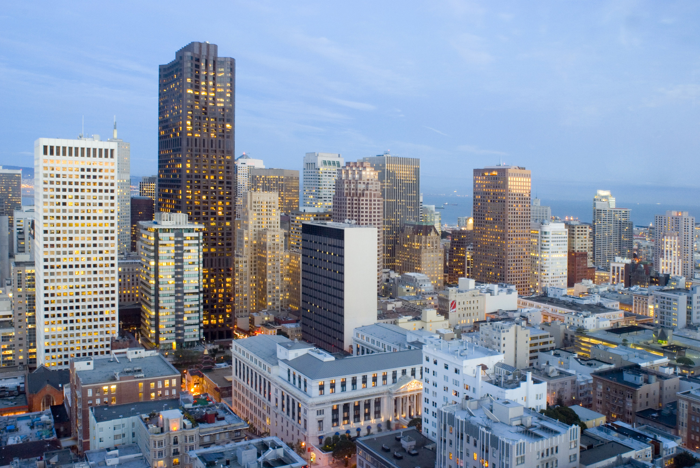
\includegraphics[height=4cm, width=1.01\textwidth]{d_content1}
        \label{fig:dpst_d_content1}
        \caption{}
	\end{subfigure}
    \hfill
    \begin{subfigure}[b]{0.24\textwidth}
		\centering
        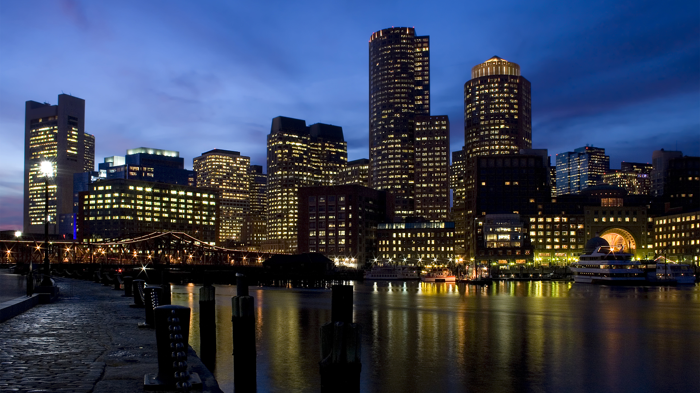
\includegraphics[height=4cm, width=1.01\textwidth]{d_style1}
        \label{fig:dpst_d_style1}
        \caption{}
	\end{subfigure}
    \hfill
    \begin{subfigure}[b]{0.24\textwidth}
		\centering
        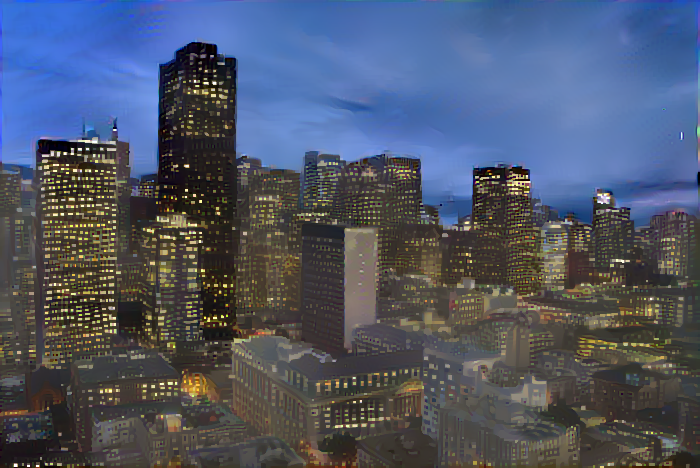
\includegraphics[height=4cm, width=1.01\textwidth]{dpst_c1s1}
        \label{fig:dpst_c1s1}
        \caption{}
	\end{subfigure}
    \hfill
    \begin{subfigure}[b]{0.24\textwidth}
		\centering
        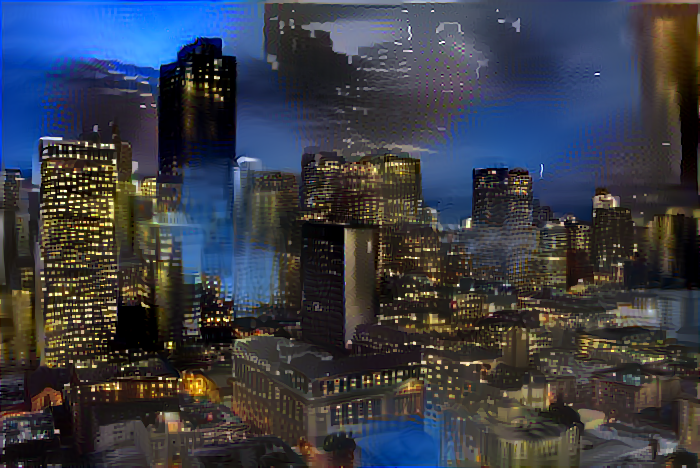
\includegraphics[height=4cm, width=1.01\textwidth]{dpst_c1s1_gatys}
        \label{fig:dpst_c1s1_gatys}
        \caption{}
	\end{subfigure}
    \caption{În această figură poza $(a)$ este poza cu conținutul pe care dorim să îl obținem, iar poza $(b)$ este poza cu stilul dorit. Poza $(c)$ a fost generată cu algoritmul din capitolul [\ref{dpst}] pe când poza $(d)$ a fost generată cu algoritmul din capitolul [\ref{anaoas}]. Se observă că dacă nu sunt folosite măști pentru a controla unde să se aplice stilul, atunci înțelesul semantic nu este păstrat, după cum se poate vedea de exemplu că părți ale cerului au fost generate pe anumite clădiri din imagine, fapt pe care nu ni-l dorim în cazul pozelor fotografice.}
\end{figure}

\newpage
\begin{figure}[h]
	\centering
    \begin{subfigure}[b]{0.24\textwidth}
		\centering
        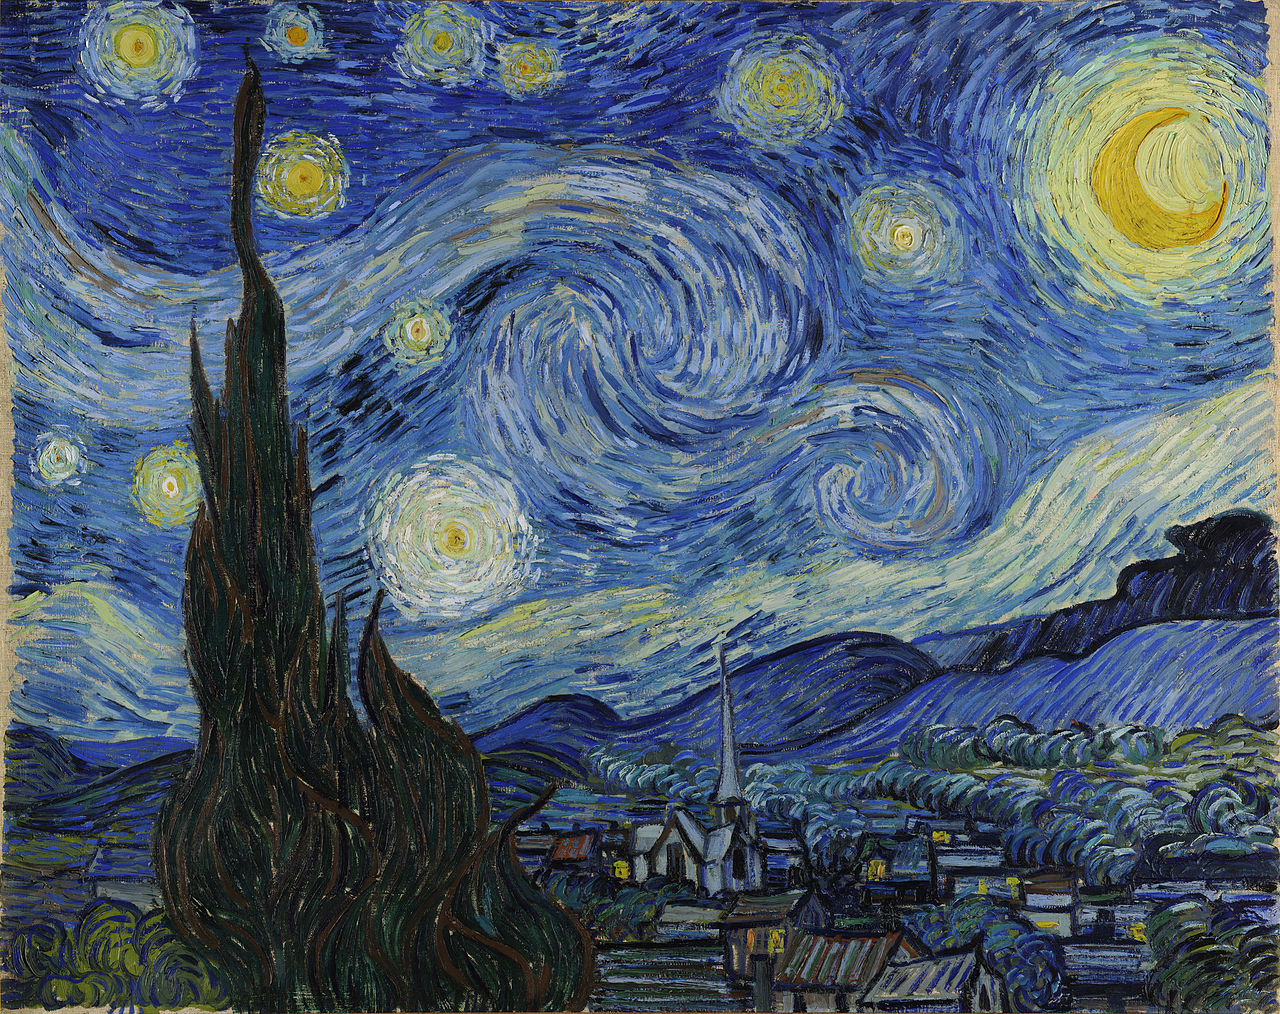
\includegraphics[height=4cm, width=1.01\textwidth]{style1}
        \label{fig:anaos_style1}
	\end{subfigure}
    \hfill
    \begin{subfigure}[b]{0.24\textwidth}
		\centering
        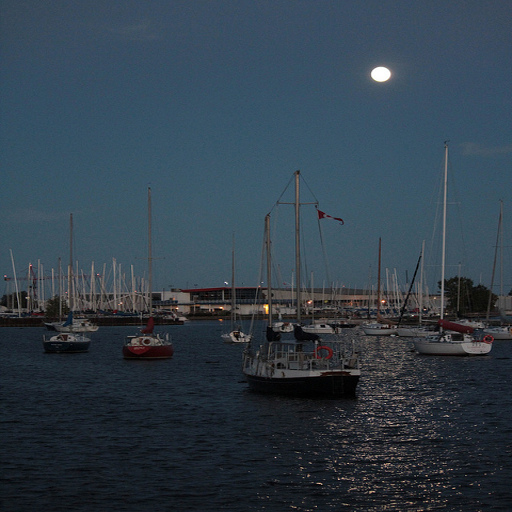
\includegraphics[height=4cm, width=1.01\textwidth]{plfrtst_c1s1_high}
        \label{fig:plfrtst_c1s1_high}
	\end{subfigure}
    \hfill
    \begin{subfigure}[b]{0.24\textwidth}
		\centering
        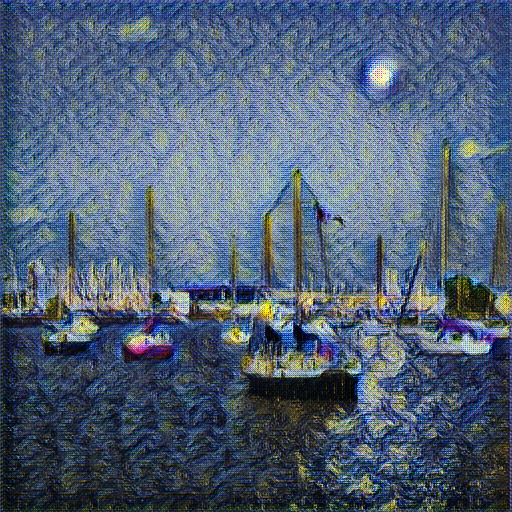
\includegraphics[height=4cm, width=1.01\textwidth]{plfrtst_c1s1_high_stil}
        \label{fig:plfrtst_c1s1_high_stil}
	\end{subfigure}
    \hfill
    \begin{subfigure}[b]{0.24\textwidth}
		\centering
        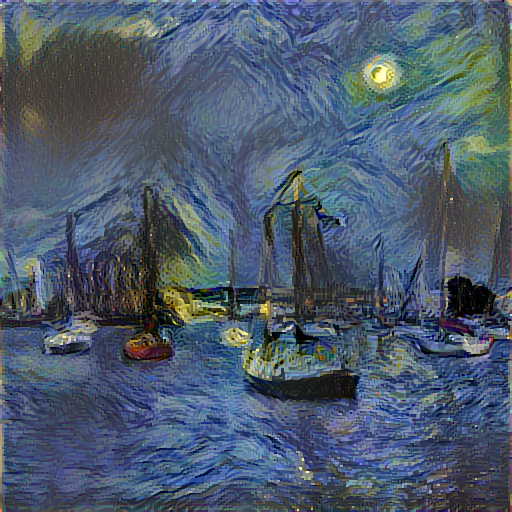
\includegraphics[height=4cm, width=1.01\textwidth]{anaoas_c1s1_high_stil}
        \label{fig:anaoas_c1s1_high_stil}
	\end{subfigure}
    \begin{subfigure}[b]{0.24\textwidth}
		\centering
        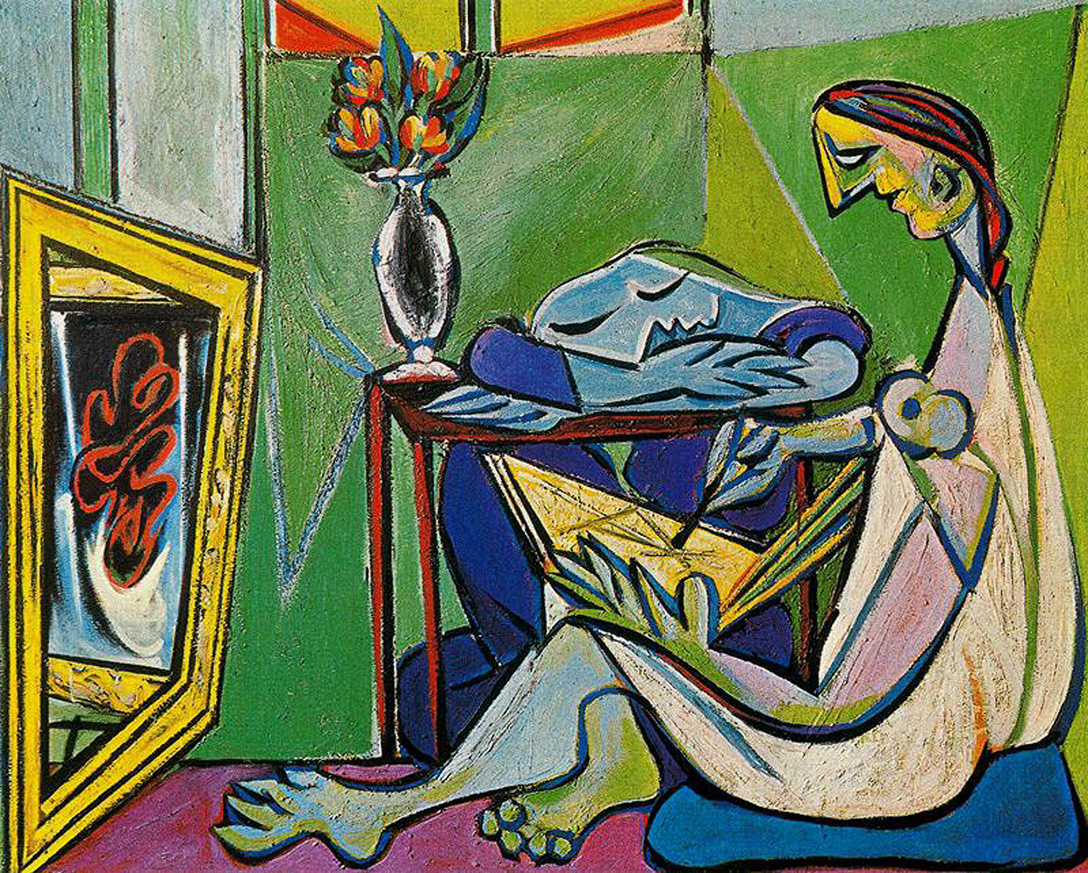
\includegraphics[height=4cm, width=1.01\textwidth]{style6}
        \label{fig:anaos_style6}
	\end{subfigure}
    \hfill
    \begin{subfigure}[b]{0.24\textwidth}
		\centering
        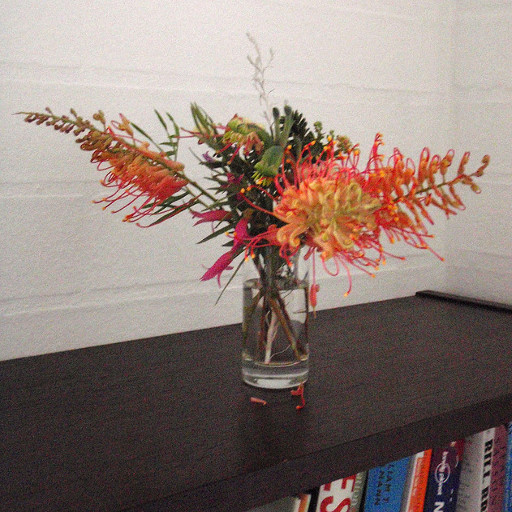
\includegraphics[height=4cm, width=1.01\textwidth]{plfrtst_c1s6_high}
        \label{fig:plfrtst_c1s6_high}
	\end{subfigure}
    \hfill
    \begin{subfigure}[b]{0.24\textwidth}
		\centering
        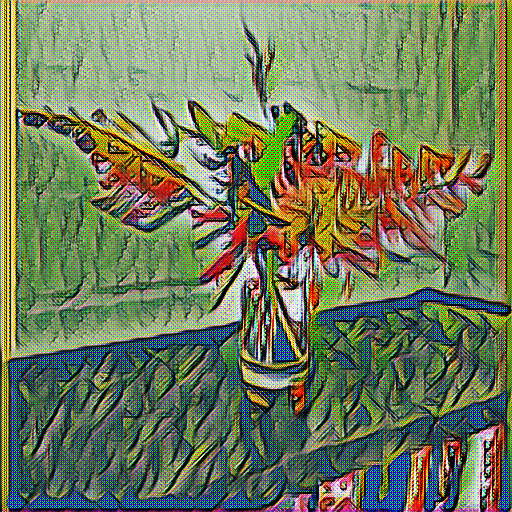
\includegraphics[height=4cm, width=1.01\textwidth]{plfrtst_c1s6_high_stil}
        \label{fig:plfrtst_c1s6_high_stil}
	\end{subfigure}
    \hfill
    \begin{subfigure}[b]{0.24\textwidth}
		\centering
        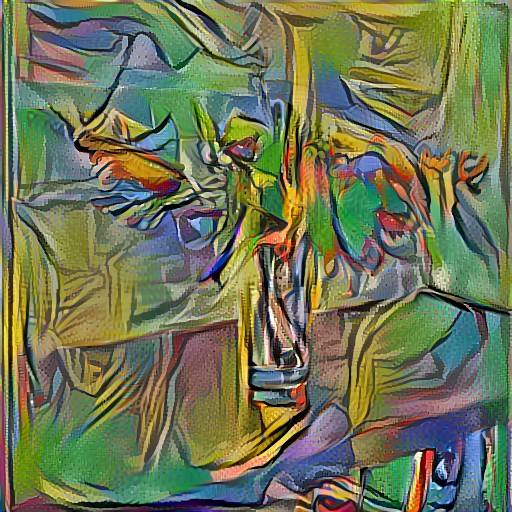
\includegraphics[height=4cm, width=1.01\textwidth]{anaoas_c1s6_high_stil}
        \label{fig:anaoas_c1s6_high_stil}
	\end{subfigure}
    \begin{subfigure}[b]{0.24\textwidth}
		\centering
        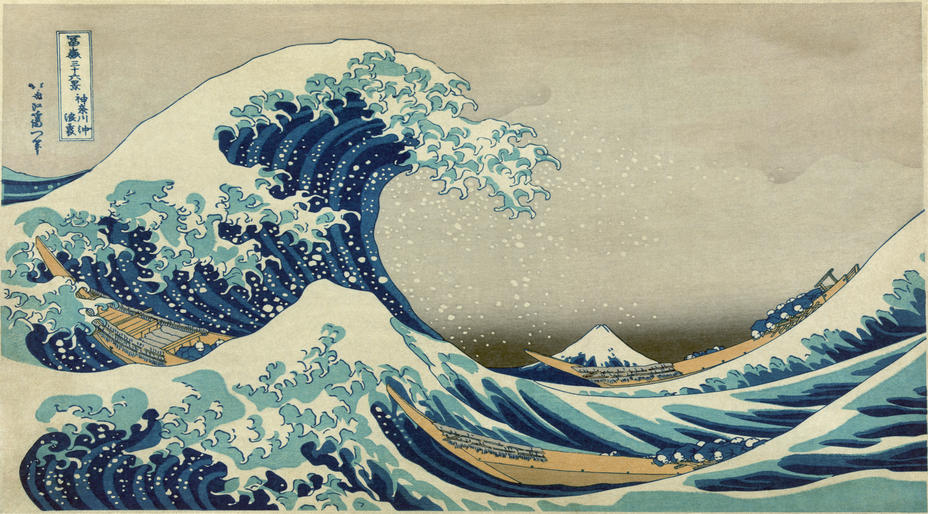
\includegraphics[height=4cm, width=1.01\textwidth]{style7}
        \label{fig:anaos_style7}
        \caption{}
	\end{subfigure}
    \hfill
    \begin{subfigure}[b]{0.24\textwidth}
		\centering
        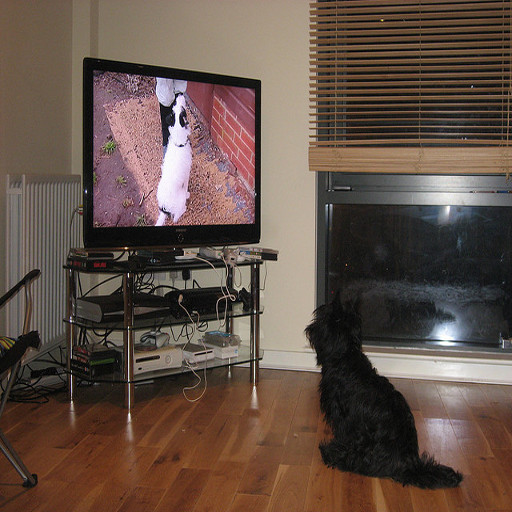
\includegraphics[height=4cm, width=1.01\textwidth]{plfrtst_c1s7_high}
        \label{fig:plfrtst_c1s7_high}
        \caption{}
	\end{subfigure}
    \hfill
    \begin{subfigure}[b]{0.24\textwidth}
		\centering
        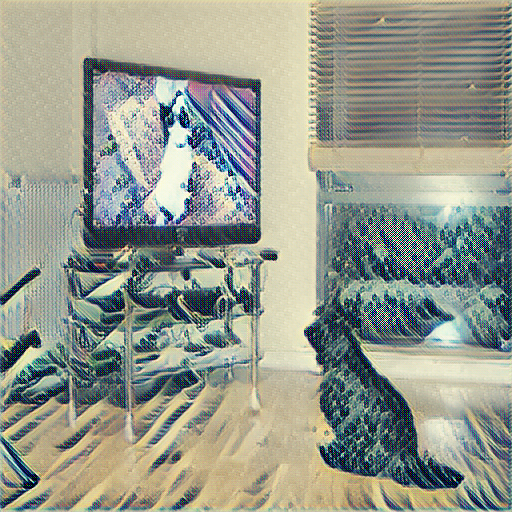
\includegraphics[height=4cm, width=1.01\textwidth]{plfrtst_c1s7_high_stil}
        \label{fig:plfrtst_c1s7_high_stil}
        \caption{}
	\end{subfigure}
    \hfill
    \begin{subfigure}[b]{0.24\textwidth}
		\centering
        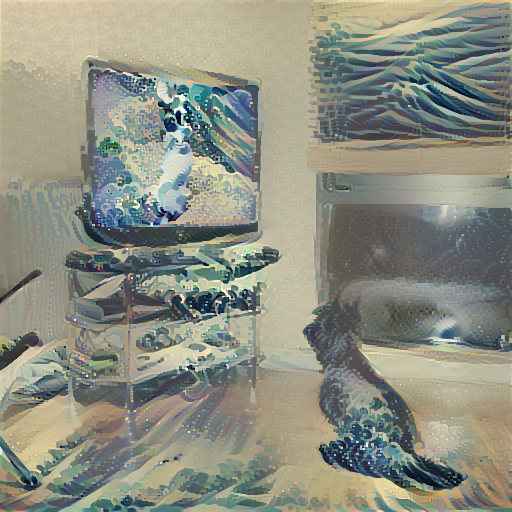
\includegraphics[height=4cm, width=1.01\textwidth]{anaoas_c1s7_high_stil}
        \label{fig:anaoas_c1s7_high_stil}
        \caption{}
	\end{subfigure}
    \caption{În această figură poza $(a)$ este poza cu conținutul pe care dorim să îl obținem, iar poza $(b)$ este poza cu stilul dorit. Pozele de pe coloana $(c)$ a fost generate cu algoritmul din capitolul [\ref{plfrtst}] pe când pozele de pe coloana $(d)$ au fost generate cu algoritmul din capitolul [\ref{anaoas}]. Se observă ca pozele generate cu cele două metode sunt aproximativ la fel, cele de pe coloana $(c)$ punând mai mult accent pe conținut, pe când cele de pe coloana $(d)$ pun accent mai mult pe stil, însă este vorba doar de preferință între cele două metode. O diferență majoră însă între cele două este timpul necesar generării unei astfel de poze. Am testat pe laptopul meu care are o placă video NVIDIA GeForce 840M și rezultatele sunt următoarele: timpul necesar pentru generarea unei poze de pe coloana $(c)$ este de aproximativ $4 secunde$, pe când timpul necesar generării unei poze de pe coloana $(d)$ pentru a obține rezultate satisfăcătoare este de aproximativ $100 de minute$, menționez că dimensiunea pozelor este de $512$ $x$ $512$ de pixeli.}
\end{figure}